\documentclass[aspectratio=169]{beamer}

% Shared Beamer settings for Applied Machine Learning lectures (UPES).
% Keep this file free of \documentclass to allow reuse via \input.

% Allow lecture sources to use shared theme/assets without copying them into each lecture folder.
% NOTE: These paths are relative to `Unit-xx/Lecture-yy/latex/` (and `Lab/Experiment-xx/latex/`).
\makeatletter
\def\input@path{{../../../_shared/}{../../../_shared/UPES-Beamer-Theme/}}
\makeatother

\usetheme{UPES}
\setbeamertemplate{navigation symbols}{}

\usepackage{amsmath}
\usepackage{amssymb}
\usepackage{booktabs}
\usepackage{graphicx}
\usepackage{hyperref}
\usepackage{xcolor}
\usepackage{listings}

% Code listings (Python-oriented for this subject).
\lstset{
  language=Python,
  basicstyle=\ttfamily\small,
  keywordstyle=\color{blue},
  commentstyle=\color{gray},
  stringstyle=\color{teal},
  showstringspaces=false,
  columns=fullflexible,
  breaklines=true
}

\usepackage{tikz}
\usetikzlibrary{arrows.meta,positioning,shapes.geometric,calc,fit,backgrounds}

% Per-slide source line (references shown on the slide itself).
\newcommand{\slidesources}[1]{%
  \vfill
  {\tiny\color{gray}\raggedright\sloppy\parbox{\linewidth}{Sources: #1}\par}%
}

% Unit-wise source strings for this subject (used by slides/notes).
% Path is relative to the lecture `latex/` folder (the compilation CWD).
% Source strings for Applied Machine Learning (CSAI2017P) — used by slides + notes.
% Prescribed texts and reference books are taken from the course syllabus.
% Support texts are the author-hosted open-access editions:
%   statlearning.com            (ISL with Python)
%   probml.github.io/pml-book   (Murphy, Probabilistic Machine Learning)
%   d2l.ai                      (Dive into Deep Learning)
%   mml-book.github.io          (Mathematics for Machine Learning)

\newcommand{\AMLRepoURL}{https://github.com/tali7c/Applied-Machine-Learning}

% --- prescribed -------------------------------------------------------------
\newcommand{\AMLPrescribed}{%
M\"uller and Guido, \textit{Introduction to Machine Learning with Python}, O'Reilly, 2016.;%
Bishop, \textit{Pattern Recognition and Machine Learning}, Springer, 2006.;%
Murphy, \textit{Machine Learning: A Probabilistic Perspective}, MIT Press, 2012.;%
Han, Kamber and Pei, \textit{Data Mining: Concepts and Techniques} (3e), Morgan Kaufmann, 2012.%
}

% --- unit-wise ---------------------------------------------------------------
\newcommand{\AMLUnitISources}{%
M\"uller and Guido, \textit{Introduction to Machine Learning with Python}, Ch. 1.;%
Bishop, \textit{Pattern Recognition and Machine Learning}, Ch. 1.;%
Murphy, \textit{Probabilistic Machine Learning: An Introduction}, MIT Press, 2022, Ch. 1.;%
Mitchell, \textit{Machine Learning}, McGraw Hill, 1997, Ch. 1.;%
Scikit-learn documentation, accessed 2026-08-04.%
}

\newcommand{\AMLUnitIISources}{%
Bishop, \textit{Pattern Recognition and Machine Learning}, \S1.5, \S4.3, \S7.1.;%
Zhang, Lipton, Li and Smola, \textit{Dive into Deep Learning}, \S3.4.;%
Shalev-Shwartz and Ben-David, \textit{Understanding Machine Learning}, Ch. 15.;%
Murphy, \textit{Probabilistic Machine Learning: An Introduction}, Ch. 5.%
}

\newcommand{\AMLUnitIIISources}{%
Zhang, Lipton, Li and Smola, \textit{Dive into Deep Learning}, Ch. 12 (Optimization Algorithms).;%
Deisenroth, Faisal and Ong, \textit{Mathematics for Machine Learning}, Ch. 7.;%
Kingma and Ba, ``Adam: A Method for Stochastic Optimization,'' ICLR 2015.;%
Ruder, ``An overview of gradient descent optimization algorithms,'' arXiv:1609.04747, 2016.%
}

\newcommand{\AMLUnitIVSources}{%
Han, Kamber and Pei, \textit{Data Mining: Concepts and Techniques} (3e), Ch. 3.;%
M\"uller and Guido, \textit{Introduction to Machine Learning with Python}, Ch. 3--4.;%
James, Witten, Hastie, Tibshirani and Taylor, \textit{An Introduction to Statistical Learning with Python}, Ch. 5--6, 12.;%
Scikit-learn documentation (preprocessing, model selection), accessed 2026-08-04.%
}

\newcommand{\AMLUnitVSources}{%
James et al., \textit{An Introduction to Statistical Learning with Python}, Ch. 3--6.;%
Bishop, \textit{Pattern Recognition and Machine Learning}, Ch. 3.;%
Deisenroth, Faisal and Ong, \textit{Mathematics for Machine Learning}, Ch. 9.;%
M\"uller and Guido, \textit{Introduction to Machine Learning with Python}, \S2.3.%
}

\newcommand{\AMLUnitVISources}{%
Han, Kamber and Pei, \textit{Data Mining: Concepts and Techniques} (3e), Ch. 8--9.;%
James et al., \textit{An Introduction to Statistical Learning with Python}, Ch. 8--9.;%
Bishop, \textit{Pattern Recognition and Machine Learning}, Ch. 4--5, 7, 14.;%
Zhang et al., \textit{Dive into Deep Learning}, Ch. 5.%
}

\newcommand{\AMLUnitVIISources}{%
Han, Kamber and Pei, \textit{Data Mining: Concepts and Techniques} (3e), Ch. 10.;%
James et al., \textit{An Introduction to Statistical Learning with Python}, Ch. 12.;%
M\"uller and Guido, \textit{Introduction to Machine Learning with Python}, \S3.5.;%
Ester, Kriegel, Sander and Xu, ``A density-based algorithm for discovering clusters (DBSCAN),'' KDD 1996.%
}

\newcommand{\AMLLabSources}{%
M\"uller and Guido, \textit{Introduction to Machine Learning with Python}, companion notebooks.;%
McKinney, \textit{Python for Data Analysis} (3e), O'Reilly, 2022.;%
Scikit-learn user guide, accessed 2026-08-04.;%
Matplotlib and Seaborn documentation, accessed 2026-08-04.%
}



\graphicspath{{../figures/}{../images/}{../../../_shared/}{../../../_shared/UPES-Beamer-Theme/}}

\title[Applied Machine Learning]{Applied Machine Learning}
\subtitle{Unit 06 -- Lecture 14: Decision Trees and Attribute Selection}
\author{Tofik Ali}
\institute{School of Computer Science, UPES Dehradun}
\date{Autumn 2026}

% ---- a compact "output" block so code and its result sit together ----------
\lstdefinestyle{outblk}{
  basicstyle=\ttfamily\scriptsize\color{black!75},
  backgroundcolor=\color{black!5}, frame=leftline, framerule=2pt,
  rulecolor=\color{black!30}, breaklines=true, columns=fullflexible,
  keepspaces=true,   % several outputs below are aligned tables
  language={},       % printed output is not Python: do not syntax-highlight it
  xleftmargin=4pt, aboveskip=1pt, belowskip=1pt, literate={-}{{-}}1}
\lstnewenvironment{outblk}{\lstset{style=outblk}}{}

\begin{document}

\UPESCoverFrame
\setcounter{framenumber}{0}

\begin{frame}
  \titlepage
  \begin{center}
    \footnotesize Entropy, information gain, ID3, and reading a tree as
    rules\\[0.25em]
    \footnotesize Topic focus: \textbf{a model made of questions, chosen by
    arithmetic}\\[0.25em]
    \footnotesize Repository: \texttt{\AMLRepoURL}
  \end{center}
  \slidesources{\AMLUnitVISources}
\end{frame}

\begin{frame}{Quick Links}
  \centering
  \hyperlink{sec:tree}{\beamerbutton{What a tree is}}\hspace{0.4em}
  \hyperlink{sec:entropy}{\beamerbutton{Entropy}}\hspace{0.4em}
  \hyperlink{sec:gain}{\beamerbutton{Information gain}}\hspace{0.4em}
  \hyperlink{sec:id3}{\beamerbutton{ID3}}\\[0.6em]
  \hyperlink{sec:rules}{\beamerbutton{Tree to rules}}\hspace{0.4em}
  \hyperlink{sec:gini}{\beamerbutton{Gini}}\hspace{0.4em}
  \hyperlink{sec:gainratio}{\beamerbutton{Gain ratio}}\hspace{0.4em}
  \hyperlink{sec:prune}{\beamerbutton{Overfitting}}\hspace{0.4em}
  \hyperlink{sec:summary}{\beamerbutton{Summary}}
\end{frame}

\begin{frame}{Agenda}
  \tableofcontents
\end{frame}

\begin{frame}[shrink=6]{How this lecture works}
  \begin{columns}[T]
    \begin{column}{0.48\textwidth}
      \begin{block}{Every idea appears twice}
        \begin{enumerate}
          \item \textbf{By hand} --- fourteen days of weather, four columns of
            words. Small enough that every logarithm can be checked with a
            pen.
          \item \textbf{In code} --- the same arithmetic, then the same
            arithmetic again inside \texttt{scikit-learn}, so you can see the
            library is doing exactly this and nothing magic.
        \end{enumerate}
      \end{block}
    \end{column}
    \begin{column}{0.48\textwidth}
      \begin{alertblock}{Commit before you look}
        Five slides ask you to predict a number before it is revealed. Write
        your guess down. Being wrong on paper is how the idea sticks.
      \end{alertblock}
    \end{column}
  \end{columns}
  \vspace{0.4em}
  \begin{center}
    \small The centrepiece is \textbf{the full ID3 computation on fourteen
    rows}: $H(S)$, the gain of all four attributes, the recursion, the tree.
    It is the most examinable arithmetic in Unit VI.
  \end{center}
\end{frame}

\begin{frame}{One table, three datasets, one seed}
  \begin{columns}[T]
    \begin{column}{0.48\textwidth}
      \begin{block}{The data}
        \small The fourteen-row play-tennis table, typed out rather than
        drawn; scikit-learn's bundled \texttt{load\_iris},
        \texttt{load\_wine} and \texttt{load\_breast\_cancer}; and one
        noisy synthetic set fixed by
        \texttt{make\_classification(\dots, random\_state=0)}. Nothing is
        downloaded.
      \end{block}
    \end{column}
    \begin{column}{0.48\textwidth}
      \begin{block}{The randomness}
        \small One seed: \texttt{np.random.default\_rng(0)} and
        \texttt{random\_state=0} in every split, shuffle and tree. Where the
        \emph{spread} is the measurement --- $2000$ entropy-vs-Gini contests,
        $200$ bootstrap root splits, $30$ repeated $70/30$ splits --- the
        seeds run $0, 1, 2, \dots$ from that same one.
      \end{block}
    \end{column}
  \end{columns}
  \vspace{0.5em}
  \begin{exampleblock}{Why this matters to you}
    \centering\small
    Every number in this deck is printed by one script. Run the code as
    written and you get the same numbers --- which is the only reason to
    believe a number on a slide.
  \end{exampleblock}
\end{frame}

\begin{frame}[shrink=5]{Where we are}
  \begin{columns}[T]
    \begin{column}{0.47\textwidth}
      \begin{block}{The previous lecture stored the data}
        $k$-nearest neighbours keeps every training row and answers a query by
        asking who is nearby. All the work happens at prediction time, and the
        explanation is ``these five rows looked like you''.
      \end{block}
      \begin{block}{This lecture stores questions instead}
        A decision tree keeps no rows at all. It keeps a sequence of tests.
        Answer them and you arrive at a prediction, and \textbf{the path you
        took is the explanation}.
      \end{block}
    \end{column}
    \begin{column}{0.49\textwidth}
      \begin{exampleblock}{Today's one question}
        Given a set of labelled rows, \emph{which question should I ask
        first?} Everything else in the lecture is machinery for answering
        that.
      \end{exampleblock}
      \begin{alertblock}{And the answer is a number}
        Measure how mixed up a set of labels is. Try every attribute. Keep the
        one that reduces the mixed-up-ness the most. That measure is
        \textbf{entropy}, the reduction is \textbf{information gain}, and the
        algorithm that repeats it is \textbf{ID3}.
      \end{alertblock}
    \end{column}
  \end{columns}
\end{frame}

% =====================================================================
\section[Trees]{What a decision tree is}
\label{sec:tree}

\begin{frame}[shrink=6]{A model made of questions}
  \begin{exampleblock}{}
    \centering\large
    Internal node $=$ a test. Branch $=$ an answer. Leaf $=$ a class label.
  \end{exampleblock}
  \vspace{0.3em}
  \begin{columns}[T]
    \begin{column}{0.48\textwidth}
      \begin{block}{To classify a new row}
        Start at the root. Answer the question. Follow the matching branch.
        Repeat until you hit a leaf. Read the label off the leaf.
      \end{block}
    \end{column}
    \begin{column}{0.48\textwidth}
      \begin{alertblock}{What is \emph{not} in that description}
        No distance. No coefficients. No requirement that anything be numeric
        --- the example this lecture is built on has four attributes and
        \textbf{every one of them is a word}.
      \end{alertblock}
    \end{column}
  \end{columns}
  \vspace{0.2em}
  \begin{center}\small
    A decision tree is a nested set of IF--THEN rules a human can read out
    loud. Every other property of trees --- no scaling needed, categorical
    data handled natively, spectacular overfitting --- \textbf{follows from
    that one sentence.}
  \end{center}
\end{frame}

\begin{frame}[shrink=6]{Drawn: a tree is a recursive partition}
  \begin{center}
    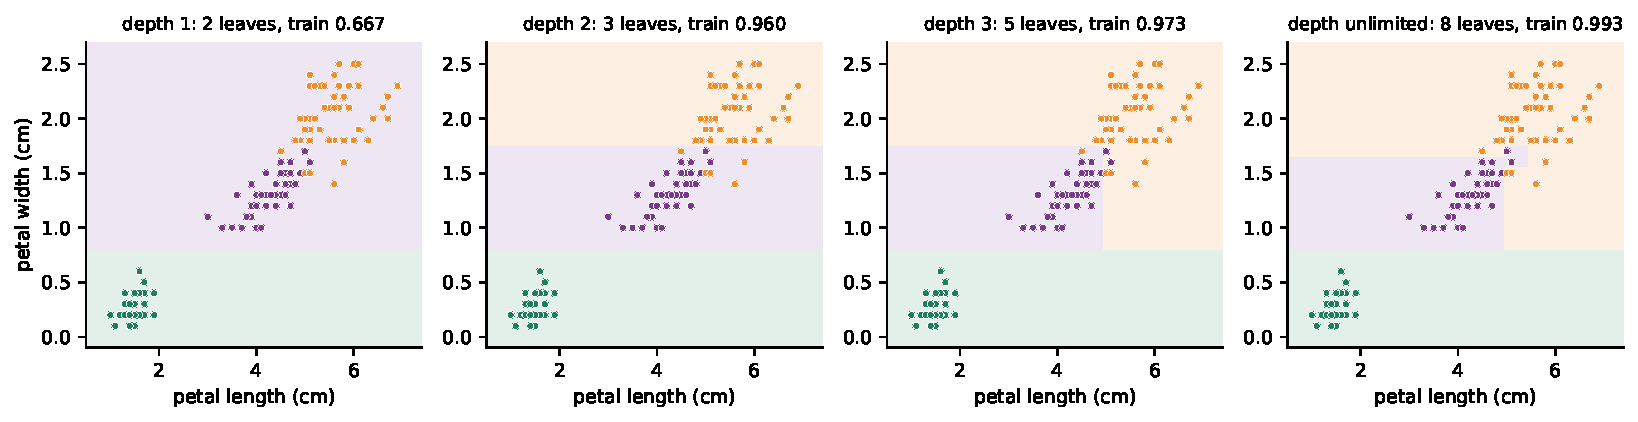
\includegraphics[width=0.96\textwidth]{partition.pdf}
  \end{center}
  \begin{center}\small
    Two features of \texttt{load\_iris}. Each question ``is $x_j \le t$?'' is
    a cut perpendicular to an axis, always inside a region an earlier cut
    produced. Depth 1 separates one species perfectly; depth 2 reaches
    $0.960$ training accuracy with three leaves; unlimited depth reaches
    $0.993$ with eight. \textbf{The thin slivers on the right are what
    overfitting looks like geometrically} --- and cross-validated, depth 2
    and unlimited depth both score $0.9267$.
  \end{center}
\end{frame}

\begin{frame}[shrink=5]{Induction is greedy, and it has to be}
  \begin{columns}[T]
    \begin{column}{0.48\textwidth}
      \begin{block}{The search space is hopeless}
        There are astronomically many trees consistent with a given table, and
        finding the smallest one is \textbf{NP-complete}.
      \end{block}
      \begin{block}{So every practical algorithm is greedy}
        Pick the single best question \emph{now}, split the data, recurse on
        each part, \textbf{never reconsider}. The family is called
        \emph{top-down induction of decision trees}.
      \end{block}
    \end{column}
    \begin{column}{0.48\textwidth}
      \begin{exampleblock}{The only thing left to choose}
        What ``best question'' means. That choice is an \textbf{attribute
        selection measure}, and Han, Kamber and Pei give three:
        \begin{itemize}\small
          \item \textbf{information gain} --- ID3
          \item \textbf{gain ratio} --- C4.5
          \item \textbf{Gini index} --- CART
        \end{itemize}
      \end{exampleblock}
      \begin{alertblock}{All three are in this lecture}
        \small Information gain comes first, because the other two are best
        understood as answers to problems it has.
      \end{alertblock}
    \end{column}
  \end{columns}
\end{frame}

\begin{frame}[fragile,shrink=16]{The table everything is built on}
Quinlan's fourteen-day weather record. Build it yourself; do not download it.
\begin{outblk}
Day  Outlook   Temperature  Humidity Wind    PlayTennis
D1   Sunny     Hot          High    Weak    No
D2   Sunny     Hot          High    Strong  No
D3   Overcast  Hot          High    Weak    Yes
D4   Rain      Mild         High    Weak    Yes
D5   Rain      Cool         Normal  Weak    Yes
D6   Rain      Cool         Normal  Strong  No
D7   Overcast  Cool         Normal  Strong  Yes
D8   Sunny     Mild         High    Weak    No
D9   Sunny     Cool         Normal  Weak    Yes
D10  Rain      Mild         Normal  Weak    Yes
D11  Sunny     Mild         Normal  Strong  Yes
D12  Overcast  Mild         High    Strong  Yes
D13  Overcast  Hot          Normal  Weak    Yes
D14  Rain      Mild         High    Strong  No
rows 14   Yes 9   No 5
Outlook      levels: Overcast, Rain, Sunny
Temperature  levels: Cool, Hot, Mild
Humidity     levels: High, Normal
Wind         levels: Strong, Weak
\end{outblk}
\onslide<2->
\begin{center}\small
  Four attributes, one class column --- and a \texttt{Day} identifier that is
  \textbf{not} an attribute. Remember it is there. A whole section of this
  lecture is about what happens when you forget.
\end{center}
\end{frame}

% =====================================================================
\section{Entropy}
\label{sec:entropy}

\begin{frame}[shrink=5]{The question entropy answers}
  \begin{columns}[T]
    \begin{column}{0.47\textwidth}
      \begin{block}{A node of the tree holds some rows}
        If every row has the same label the node is \textbf{pure} and there is
        nothing left to learn. If the labels are evenly split the node is as
        \textbf{impure} as it can be: knowing a row landed here tells you
        nothing.
      \end{block}
      \begin{alertblock}{So we want a number that is}
        \small $0$ in the first case, maximal in the second, and smooth in
        between.
      \end{alertblock}
    \end{column}
    \begin{column}{0.49\textwidth}
      \begin{exampleblock}{Shannon's answer}
        \[
          H \;=\; -\sum_{i=1}^{m} p_i \log_2 p_i ,
          \qquad 0\log_2 0 = 0 .
        \]
      \end{exampleblock}
      \begin{block}{Two names, one formula}
        \small Han, Kamber and Pei write this $\mathrm{Info}(D)$ and call it
        \emph{the expected information needed to classify a tuple in $D$}.
        Both names appear in examination papers. \textbf{They are the same
        thing.}
      \end{block}
    \end{column}
  \end{columns}
\end{frame}

\begin{frame}[shrink=8]{By hand: entropy at the two extremes}
  \begin{columns}[T]
    \begin{column}{0.48\textwidth}
      \begin{block}{A pure node}
        All rows ``Yes'', so $p_{\text{Yes}} = 1$, $p_{\text{No}} = 0$:
        \[ H = -1\log_2 1 - 0\log_2 0 = \mathbf{0}. \]
        No questions needed. You already know.
      \end{block}
      \begin{block}{An evenly split binary node}
        \[
          H = -\tfrac12\log_2\tfrac12 - \tfrac12\log_2\tfrac12
            = \tfrac12 + \tfrac12 = \mathbf{1}\ \text{bit}.
        \]
        Exactly one yes/no question, which is obviously right.
      \end{block}
    \end{column}
    \begin{column}{0.48\textwidth}
      \begin{block}{$m$ equally likely classes}
        \[
          H = -\sum_{i=1}^{m}\tfrac1m\log_2\tfrac1m = \log_2 m .
        \]
        Three classes give $1.5850$, four give $2$, ten give $3.3219$.
        \textbf{This is the ceiling.}
      \end{block}
      \begin{alertblock}{$H$ is symmetric}
        \small $9$ Yes and $5$ No has exactly the same entropy as $5$ Yes and
        $9$ No. Entropy measures \emph{how mixed}, not \emph{which class
        dominates}. Two nodes with equal entropy can predict opposite labels.
      \end{alertblock}
    \end{column}
  \end{columns}
\end{frame}

\begin{frame}[fragile,shrink=10]{The same thing in code}
\begin{lstlisting}
def H(p):
    return 0.0 if p in (0.0, 1.0) else -(p*log2(p) + (1-p)*log2(1-p))
\end{lstlisting}
\begin{outblk}
entropy of a two-class node, H(p) = -p log2 p - (1-p) log2 (1-p)
   p = 0.0000    H = 0.0000  pure
   p = 0.0500    H = 0.2864
   p = 0.1000    H = 0.4690
   p = 0.2500    H = 0.8113
   p = 0.3333    H = 0.9183
   p = 0.5000    H = 1.0000  MAXIMUM
   p = 0.6667    H = 0.9183
   p = 0.7500    H = 0.8113
   p = 0.9000    H = 0.4690
   p = 1.0000    H = 0.0000  pure
\end{outblk}
\onslide<2->
\begin{outblk}
uniform over k classes: H = log2(k)
   k =  2   H = 1.0000   log2(k) = 1.0000
   k =  3   H = 1.5850   log2(k) = 1.5850
   k =  4   H = 2.0000   log2(k) = 2.0000
   k =  8   H = 3.0000   log2(k) = 3.0000
   k = 10   H = 3.3219   log2(k) = 3.3219
\end{outblk}
\end{frame}

\begin{frame}[fragile,shrink=10]{Why the logarithm, and why base two}
Think of it as a coding problem. A label of probability $p$ deserves
$\log_2(1/p)$ bits, and $H$ is the average of those costs. So $H$ is in
\textbf{bits}: the average number of yes/no questions to pin down one label.
\begin{outblk}
why base 2: H is the average number of yes/no questions per message
    2 equally likely messages -> log2(2) = 1.0 bits, and 1 yes/no questions do identify one
    4 equally likely messages -> log2(4) = 2.0 bits, and 2 yes/no questions do identify one
    8 equally likely messages -> log2(8) = 3.0 bits, and 3 yes/no questions do identify one
   16 equally likely messages -> log2(16) = 4.0 bits, and 4 yes/no questions do identify one
a biased two-class source, 1000 draws at p(Yes) = 0.9
   observed p(Yes) 0.9040   H 0.4562 bits per draw
   a naive 1-bit-per-draw code costs 1000 bits; the entropy bound is 456
\end{outblk}
\onslide<2->
\begin{alertblock}{The last two lines are the whole definition}
  \footnotesize A thousand labels that are $90\%$ ``Yes'' fit in $456$ bits
  rather than $1000$, because they are predictable. \textbf{Entropy measures
  unpredictability, and a node of a tree is exactly a place where we want the
  labels to be predictable.} Base $e$ gives nats, base ten gives hartleys ---
  every comparison in this lecture comes out the same.
\end{alertblock}
\end{frame}

\begin{frame}[shrink=6]{Drawn: the shape of the three impurity measures}
  \begin{center}
    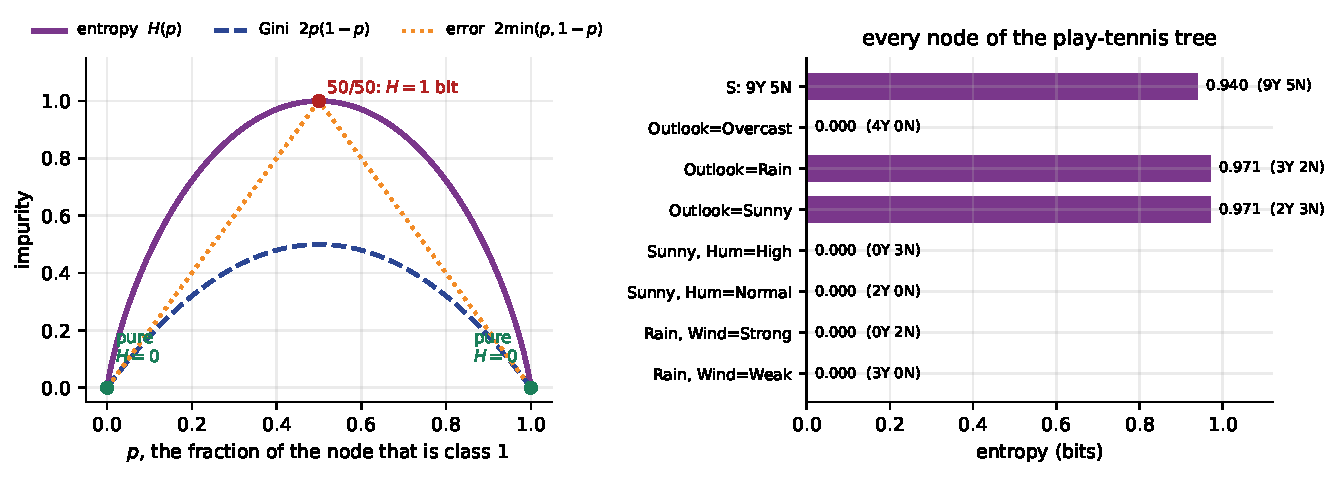
\includegraphics[width=0.92\textwidth]{entropy.pdf}
  \end{center}
  \begin{center}\small
    Left: binary entropy, with Gini and the misclassification error rescaled
    to the same peak. All three are zero at the ends and maximal at
    $p = \tfrac12$; \textbf{the error rate is flat where the other two still
    discriminate}, which is why it makes a poor splitting criterion. Right:
    every node of the tree we are about to build, in creation order --- root
    at $0.9403$, two children at $0.9710$, and all five leaves exactly $0$.
  \end{center}
\end{frame}

% =====================================================================
\section[IG]{Information gain}
\label{sec:gain}

\begin{frame}[shrink=6]{Two equations, and that is the whole idea}
  \begin{exampleblock}{The impurity that survives a split}
    \[
      \mathrm{Info}_A(S) \;=\; \sum_{v \in \mathrm{values}(A)}
        \frac{|S_v|}{|S|}\, H(S_v)
      \qquad\text{(weighted average of the children)}
    \]
  \end{exampleblock}
  \begin{exampleblock}{What the split removed}
    \[
      \mathrm{Gain}(S, A) \;=\; H(S) - \mathrm{Info}_A(S)
    \]
  \end{exampleblock}
  \vspace{0.2em}
  \begin{columns}[T]
    \begin{column}{0.48\textwidth}
      \begin{block}{Two facts that make it sensible}
        \small $\mathrm{Gain} \ge 0$ always --- splitting cannot raise the
        weighted average entropy. And $\mathrm{Gain} = H(S)$ exactly when
        every child is pure.
      \end{block}
    \end{column}
    \begin{column}{0.48\textwidth}
      \begin{alertblock}{Say it in words}
        \small Gain is \textbf{the number of bits of uncertainty about the
        class that asking about $A$ removes}. Largest gain $=$ the question
        that tells you the most.
      \end{alertblock}
    \end{column}
  \end{columns}
\end{frame}

\begin{frame}[fragile,shrink=8]{By hand: $H(S)$ for the fourteen days}
Nine ``Yes'', five ``No'', so $p_{\text{Yes}} = 9/14 = 0.642857$ and
$p_{\text{No}} = 5/14 = 0.357143$. The logarithms are
$\log_2 0.642857 = -0.637430$ and $\log_2 0.357143 = -1.485427$.
\[
  H(S) = 0.642857 \cdot 0.637430 + 0.357143 \cdot 1.485427
       = 0.409776 + 0.530510 = \mathbf{0.940286}\ \text{bits}
\]
\begin{outblk}
S has 9 Yes and 5 No out of 14
H(S) = -(9/14)log2(9/14) - (5/14)log2(5/14)
     = -(0.642857)(-0.637430) - (0.357143)(-1.485427)
     = 0.409776 + 0.530510 = 0.940286 bits
Gini(S) = 1 - (9/14)^2 - (5/14)^2 = 0.459184
\end{outblk}
\onslide<2->
\begin{alertblock}{Predict first \#1 --- write your answer down now}
  \footnotesize \texttt{Outlook} splits the fourteen rows $4/5/5$,
  \texttt{Temperature} $4/4/6$, \texttt{Humidity} $7/7$, \texttt{Wind} $6/8$.
  \textbf{Rank all four by information gain, and name the winner}, before we
  compute a single one of them. Keep the paper: we come back to it in four
  slides.
\end{alertblock}
\end{frame}

\begin{frame}[shrink=5]{By hand: $\mathrm{Gain}(S, \texttt{Outlook})$, slowly}
  \begin{center}\small
  \begin{tabular}{@{}lrrrl@{}}
    \toprule
    value & rows & Yes & No & entropy of that child\\
    \midrule
    \texttt{Overcast} & $4$ & $4$ & $0$ & $H = -1\log_2 1 = 0$\quad(pure)\\
    \texttt{Rain}     & $5$ & $3$ & $2$ &
      $H = -\tfrac35\log_2\tfrac35 - \tfrac25\log_2\tfrac25 = 0.970951$\\
    \texttt{Sunny}    & $5$ & $2$ & $3$ &
      $H = -\tfrac25\log_2\tfrac25 - \tfrac35\log_2\tfrac35 = 0.970951$\\
    \bottomrule
  \end{tabular}
  \end{center}
  The last two are equal: $2$ Yes out of $5$ and $3$ Yes out of $5$ are
  equally mixed. Now the weighted average, then the subtraction:
  \[
    \mathrm{Info}_{\texttt{Outlook}}(S)
      = \tfrac{4}{14}(0) + \tfrac{5}{14}(0.970951) + \tfrac{5}{14}(0.970951)
      = \tfrac{10}{14}\times 0.970951 = 0.693536
  \]
  \[
    \boxed{\ \mathrm{Gain}(S, \texttt{Outlook}) = 0.940286 - 0.693536
      = \mathbf{0.246750}\ }
  \]
\end{frame}

\begin{frame}[fragile,shrink=6]{The same thing in code}
\begin{lstlisting}
def info_after(rows, attr):
    n = len(rows)
    return sum(len(sub)/n * entropy(sub) for _, sub in partition(rows, attr))
print(entropy(TENNIS) - info_after(TENNIS, "Outlook"))
\end{lstlisting}
\begin{outblk}
Information gain of Outlook, step by step
   Outlook = Overcast    4 rows  4 Yes 0 No   H = 0.000000
   Outlook = Rain        5 rows  3 Yes 2 No   H = 0.970951
   Outlook = Sunny       5 rows  2 Yes 3 No   H = 0.970951
   Info_Outlook(S) = (4/14)(0.0000) + (5/14)(0.9710) + (5/14)(0.9710)
                   = 0.693536
   Gain(S, Outlook) = 0.940286 - 0.693536 = 0.246750
\end{outblk}
\onslide<2->
\begin{center}\small
  Line for line, the same six numbers we put on the board. \textbf{Three
  lines of Python and a dictionary of subsets is the entire attribute
  selection measure} --- there is nothing else in it.
\end{center}
\end{frame}

\begin{frame}[shrink=10]{By hand: the other three at speed}
Same three steps each time: entropy of every child, weighted average,
subtract from $H(S)$.
\begin{center}\small
\begin{tabular}{@{}l l l l r@{}}
  \toprule
  attribute & \multicolumn{3}{c}{entropy of each child} &
    $\mathrm{Info}_A(S)$\\
  \midrule
  \texttt{Temperature} $4/4/6$ & \texttt{Cool} $0.811278$
    & \texttt{Hot} $1.000000$ & \texttt{Mild} $0.918296$ & $0.911063$\\
  \texttt{Humidity} $7/7$ & \texttt{High} $0.985228$
    & \texttt{Normal} $0.591673$ & & $0.788450$\\
  \texttt{Wind} $6/8$ & \texttt{Strong} $1.000000$
    & \texttt{Weak} $0.811278$ & & $0.892159$\\
  \bottomrule
\end{tabular}
\end{center}
The middle column is the arithmetic, so do one of them in full:
\[
  \mathrm{Info}_{\texttt{Temperature}}
    = \tfrac{4}{14}(0.811278) + \tfrac{4}{14}(1.000000)
    + \tfrac{6}{14}(0.918296) = 0.911063
\]
\onslide<2->
\begin{center}
  Subtract each from $H(S) = 0.940286$:\ \
  $\mathrm{Gain}(\texttt{Temperature}) = \mathbf{0.029223}$,\ \
  $\mathrm{Gain}(\texttt{Humidity}) = \mathbf{0.151836}$,\ \
  $\mathrm{Gain}(\texttt{Wind}) = \mathbf{0.048127}$.
\end{center}
\end{frame}

\begin{frame}[fragile,shrink=10]{All three, machine-checked}
\begin{outblk}
Information gain of Temperature
   Temperature = Cool     4 rows  3 Yes 1 No   H = 0.811278
   Temperature = Hot      4 rows  2 Yes 2 No   H = 1.000000
   Temperature = Mild     6 rows  4 Yes 2 No   H = 0.918296
   Info_Temperature(S) = 0.911063     Gain = 0.940286 - 0.911063 = 0.029223
Information gain of Humidity
   Humidity    = High     7 rows  3 Yes 4 No   H = 0.985228
   Humidity    = Normal   7 rows  6 Yes 1 No   H = 0.591673
   Info_Humidity(S) = 0.788450     Gain = 0.940286 - 0.788450 = 0.151836
Information gain of Wind
   Wind        = Strong   6 rows  3 Yes 3 No   H = 1.000000
   Wind        = Weak     8 rows  6 Yes 2 No   H = 0.811278
   Info_Wind(S) = 0.892159     Gain = 0.940286 - 0.892159 = 0.048127
\end{outblk}
\onslide<2->
\begin{center}\small
  Twelve child entropies, three weighted averages, three subtractions. Every
  number matches the board. \textbf{Now look at your ranking.}
\end{center}
\end{frame}

\begin{frame}[fragile,shrink=6]{Predict first \#1 --- the reveal}
Four attributes, four gains. You wrote down a ranking four slides ago.
\begin{center}
  \textbf{Which one does ID3 put at the root, and by how much?}
\end{center}
\vspace{0.2em}
\onslide<2->
\begin{outblk}
attribute      Info_A(S)     Gain     rank
Outlook        0.693536   0.246750   1
Temperature    0.911063   0.029223   4
Humidity       0.788450   0.151836   2
Wind           0.892159   0.048127   3
ID3 splits the root on Outlook
runner-up Humidity is behind by 0.094914
\end{outblk}
\onslide<3->
\begin{center}\small
  Most people get the winner. Very few get \texttt{Temperature} in last place
  --- it \emph{feels} like the most relevant thing about a day of tennis, and
  it is the \textbf{worst} of the four questions to ask first.
\end{center}
\end{frame}

\begin{frame}[shrink=6]{Drawn: where the gain comes from}
  \begin{center}
    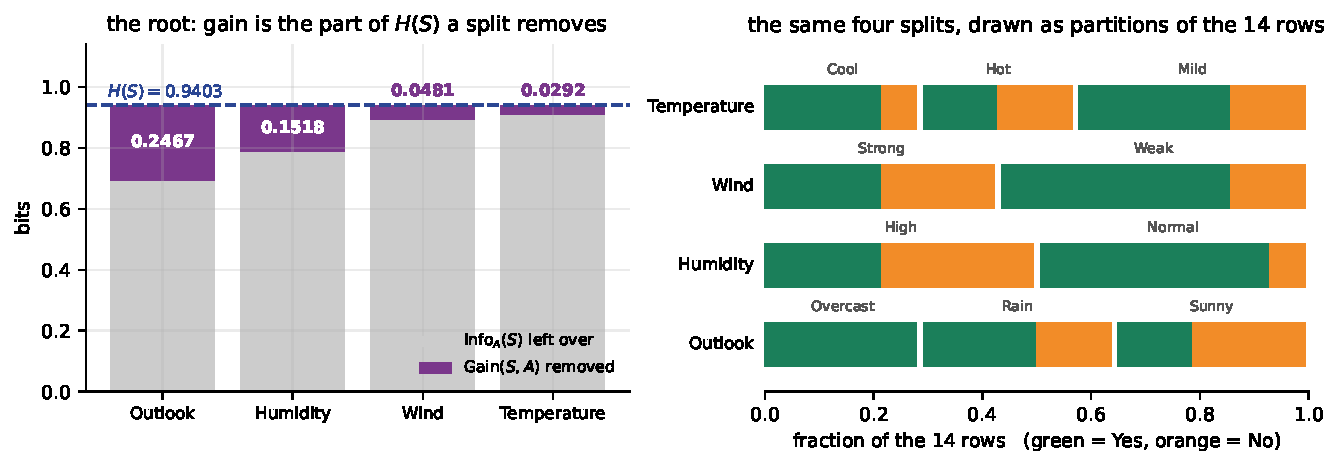
\includegraphics[width=0.96\textwidth]{tennisgain.pdf}
  \end{center}
  \begin{center}\small
    Left: each bar is $H(S) = 0.9403$ split into the part the question removes
    (purple, the gain) and the part it leaves behind (grey,
    $\mathrm{Info}_A(S)$). Right: the same four splits as partitions of the
    fourteen rows, green Yes and orange No. \textbf{The \texttt{Overcast}
    block is entirely green} --- that is where \texttt{Outlook}'s gain comes
    from. Every \texttt{Temperature} block is a mixture, which is why its gain
    is $0.0292$.
  \end{center}
\end{frame}

\begin{frame}[shrink=6]{Why \texttt{Outlook} wins --- and the commonest mistake}
  \begin{exampleblock}{The reason is one number}
    \centering
    \texttt{Outlook} is the \textbf{only attribute with a pure child}. Four
    \texttt{Overcast} days, four ``Yes'', entropy $0$.
  \end{exampleblock}
  \vspace{0.2em}
  \begin{columns}[T]
    \begin{column}{0.48\textwidth}
      \begin{block}{Read the definition again}
        \small An attribute earns gain by producing children that are less
        mixed than the parent, and \textbf{a pure child is the most any child
        can contribute}. That is the sentence to reproduce in an examination.
      \end{block}
    \end{column}
    \begin{column}{0.48\textwidth}
      \begin{alertblock}{Do not compare $\mathrm{Info}_A(S)$ and pick the largest}
        \small You want the \emph{smallest} $\mathrm{Info}$, equivalently the
        \emph{largest} gain. This sign error is the single commonest mistake
        in the examination, and it hands you \texttt{Temperature} --- the
        worst of the four.
      \end{alertblock}
    \end{column}
  \end{columns}
\end{frame}

% =====================================================================
\section{The ID3 algorithm}
\label{sec:id3}

\begin{frame}[shrink=8]{ID3 --- Iterative Dichotomiser 3, Quinlan 1986}
  \begin{block}{\textbf{ID3}$(S, \text{attributes})$}
    \begin{enumerate}\small
      \item If every row of $S$ has the same class $c$, return a leaf
        labelled $c$.
      \item If \text{attributes} is empty, return a leaf labelled with the
        \textbf{majority} class of $S$.
      \item Otherwise let $A^\star = \arg\max_A \mathrm{Gain}(S, A)$.
      \item Create a node testing $A^\star$. For each value $v$ of $A^\star$:
        let $S_v$ be the rows with $A^\star = v$; if $S_v$ is empty attach a
        leaf with the majority class of $S$; otherwise attach
        \textbf{ID3}$(S_v, \text{attributes}\setminus\{A^\star\})$.
      \item Return the node.
    \end{enumerate}
  \end{block}
  \begin{columns}[T]
    \begin{column}{0.31\textwidth}
      \begin{alertblock}{Used once per path}
        \scriptsize After splitting on $A$, every row below has the same
        value of $A$. A second split would be useless.
      \end{alertblock}
    \end{column}
    \begin{column}{0.31\textwidth}
      \begin{alertblock}{Splits are multiway}
        \scriptsize $k$ values give $k$ branches, not two. CART does not do
        this, and it matters.
      \end{alertblock}
    \end{column}
    \begin{column}{0.31\textwidth}
      \begin{alertblock}{No pruning at all}
        \scriptsize It grows until every leaf is pure or the attributes run
        out. That is a problem, and it has its own section.
      \end{alertblock}
    \end{column}
  \end{columns}
\end{frame}

\begin{frame}[fragile,shrink=8]{Step 3, by hand: the \texttt{Sunny} branch}
Five \texttt{Sunny} days: D1, D2, D8 (No) and D9, D11 (Yes). Two Yes, three
No, so $H = 0.970951$. \texttt{Outlook} is used up; three attributes remain.
\begin{outblk}
Outlook = Sunny    : 5 rows, 2 Yes 3 No, H = 0.970951  -> recurse
   Gain(S_sunny, Temperature) = 0.970951 - 0.400000 = 0.570951
   Gain(S_sunny, Humidity   ) = 0.970951 - 0.000000 = 0.970951
   Gain(S_sunny, Wind       ) = 0.970951 - 0.950978 = 0.019973
   winner: Humidity, and it is a PERFECT split
      Humidity = High    3 rows  0 Yes 3 No   H = 0.0000
      Humidity = Normal  2 rows  2 Yes 0 No   H = 0.0000
\end{outblk}
\onslide<2->
\begin{alertblock}{$0.970951$ is the \emph{entire} entropy of the node}
  \footnotesize $\mathrm{Gain} = H(S_{\text{sunny}})$ means
  $\mathrm{Info} = 0$ means \textbf{both children are pure}, so the branch is
  finished in one step. Three high-humidity sunny days: no tennis. Two
  normal-humidity sunny days: tennis.
\end{alertblock}
\end{frame}

\begin{frame}[fragile,shrink=8]{Predict first \#2 --- the \texttt{Rain} branch}
Five \texttt{Rain} days: D4, D5, D10 (Yes) and D6, D14 (No). Three Yes, two
No, so again $H = 0.970951$. Three attributes left.
\begin{center}
  \textbf{Which one does ID3 choose here --- and is it perfect too?}
\end{center}
\vspace{0.2em}
\onslide<2->
\begin{outblk}
Outlook = Rain     : 5 rows, 3 Yes 2 No, H = 0.970951  -> recurse
   Gain(S_rain, Temperature) = 0.970951 - 0.950978 = 0.019973
   Gain(S_rain, Humidity   ) = 0.970951 - 0.950978 = 0.019973
   Gain(S_rain, Wind       ) = 0.970951 - 0.000000 = 0.970951
   winner: Wind, and it is a PERFECT split
      Wind = Strong  2 rows  0 Yes 2 No   H = 0.0000
      Wind = Weak    3 rows  3 Yes 0 No   H = 0.0000
\end{outblk}
\onslide<3->
\begin{center}\small
  Rain and a strong wind: no tennis. Rain and a weak wind: tennis. And note
  \texttt{Temperature} and \texttt{Humidity} \textbf{tie} at $0.019973$ ---
  ties happen, and an implementation must break them somehow, usually by
  attribute order.
\end{center}
\end{frame}

\begin{frame}[fragile,shrink=10]{The whole algorithm, in nine lines}
\begin{lstlisting}
def id3(rows, attrs):
    yes, no = counts(rows)
    if yes == 0 or no == 0:                 # pure -> leaf
        return Leaf("Yes" if yes else "No")
    if not attrs:                           # out of attributes -> majority
        return Leaf("Yes" if yes >= no else "No")
    best = max(attrs, key=lambda a: gain(rows, a))
    return Node(best, {v: id3(sub, [a for a in attrs if a != best])
                       for v, sub in partition(rows, best)})
\end{lstlisting}
\begin{outblk}
[9 Yes, 5 No  H=0.9403]  split on Outlook (gain 0.2467)
   Outlook=Overcast: [4 Yes, 0 No  H=0.0000] --> Yes
   Outlook=Rain: [3 Yes, 2 No  H=0.9710]  split on Wind (gain 0.9710)
      Wind=Strong: [0 Yes, 2 No  H=0.0000] --> No
      Wind=Weak: [3 Yes, 0 No  H=0.0000] --> Yes
   Outlook=Sunny: [2 Yes, 3 No  H=0.9710]  split on Humidity (gain 0.9710)
      Humidity=High: [0 Yes, 3 No  H=0.0000] --> No
      Humidity=Normal: [2 Yes, 0 No  H=0.0000] --> Yes
leaves: 5
\end{outblk}
\end{frame}

\begin{frame}[shrink=6]{Drawn: the tree ID3 builds}
  \begin{center}
    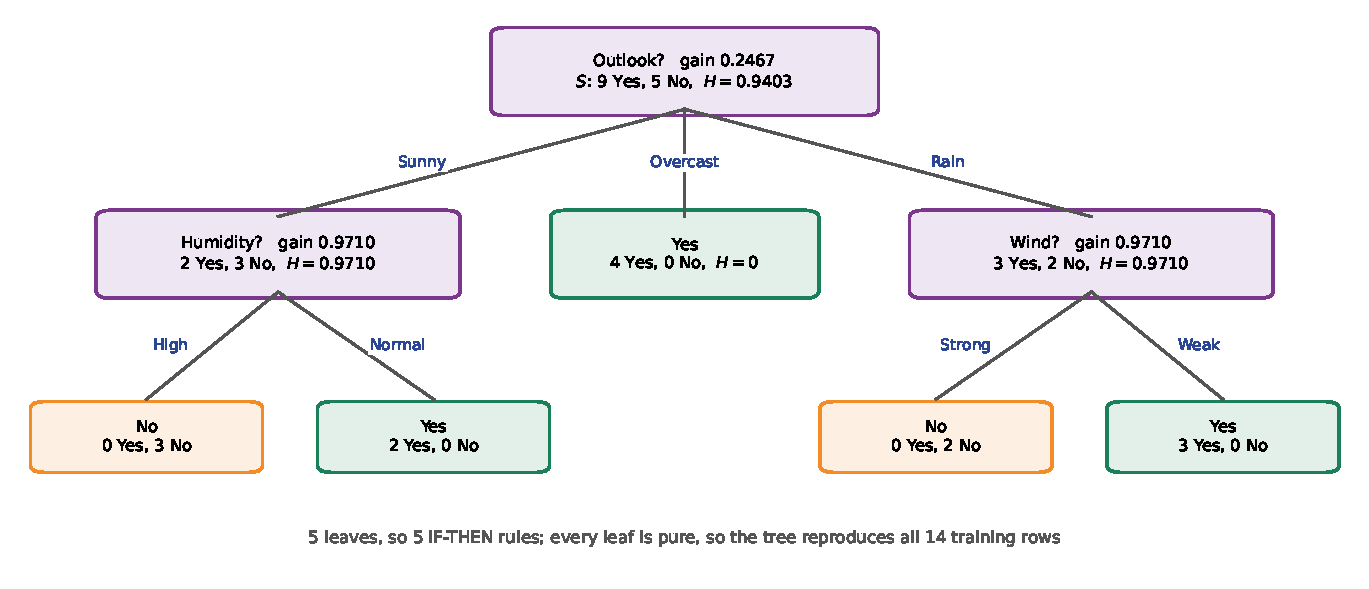
\includegraphics[width=0.94\textwidth]{tennistree.pdf}
  \end{center}
  \begin{center}\small
    Class counts, entropy and the winning gain at every node. Depth 2, five
    leaves, every leaf pure. \textbf{\texttt{Temperature} never appears} ---
    not because temperature is irrelevant to tennis, but because \emph{given}
    the outlook, humidity and wind already account for these fourteen days.
    A greedy algorithm answers ``what is the best question to ask next'', not
    ``which variables matter''.
  \end{center}
\end{frame}

\begin{frame}[fragile,shrink=8]{And if the attribute is a number?}
ID3 as stated is categorical only. C4.5 and CART turn a numeric attribute
into a binary one: sort the distinct values, take the midpoint of each
adjacent pair as a candidate threshold, and score $x \le t$ against $x > t$
with the \emph{same} formula. With $d$ distinct values, $d-1$ candidates.
\begin{lstlisting}
vals  = np.unique(petal_length)
cands = (vals[:-1] + vals[1:]) / 2          # the midpoints
best  = max(cands, key=lambda t: gain_of_threshold(t))
\end{lstlisting}
\begin{outblk}
a continuous attribute: where does the threshold come from?
   43 distinct petal-length values -> 42 candidate midpoints
   H(all 150 rows, setosa vs rest) = 0.918296
   best midpoint 2.45 cm, gain 0.918296  (a perfect split)
   scikit-learn's threshold: 2.45  -- the same number
\end{outblk}
\onslide<2->
\begin{center}\small
  Forty-two candidates, one of them perfect, and the library lands on the
  same $2.45$ cm. One asymmetry to remember: \textbf{a numeric attribute can
  be split again further down at a different threshold}; a categorical one
  cannot.
\end{center}
\end{frame}

\begin{frame}[fragile,shrink=18]{\texttt{scikit-learn} implements CART, not ID3}
Same fourteen rows, one-hot encoded because it will not take strings, with
\texttt{criterion="entropy"}.
\begin{lstlisting}
t = DecisionTreeClassifier(criterion="entropy", random_state=0).fit(X, y)
print(export_text(t, feature_names=names))
\end{lstlisting}
\begin{outblk}
|--- Outlook=Overcast <= 0.50
|   |--- Humidity=Normal <= 0.50
|   |   |--- Outlook=Rain <= 0.50
|   |   |   |--- class: 0
|   |   |--- Outlook=Rain >  0.50
|   |   |   |--- Wind=Strong <= 0.50
|   |   |   |   |--- class: 1
|   |   |   |--- Wind=Strong >  0.50
|   |   |   |   |--- class: 0
|   |--- Humidity=Normal >  0.50
|   |   |--- Wind=Weak <= 0.50
|   |   |   |--- Temperature=Cool <= 0.50
|   |   |   |   |--- class: 1
|   |   |   |--- Temperature=Cool >  0.50
|   |   |   |   |--- class: 0
|   |   |--- Wind=Weak >  0.50
|   |   |   |--- class: 1
|--- Outlook=Overcast >  0.50
|   |--- class: 1
depth 4, leaves 7, training accuracy 1.0000
our ID3 tree: depth 2, leaves 5, training accuracy 1.0000
\end{outblk}
\end{frame}

\begin{frame}[fragile,shrink=8]{Why it is a different tree --- and it is only one thing}
\begin{outblk}
root feature: Outlook=Overcast   (root impurity 0.940286, matches H(S) = 0.940286)
the binary questions available at the root, scored by information gain:
   Outlook=Overcast       gain 0.226000
   Humidity=Normal        gain 0.151836
   Humidity=High          gain 0.151836
   Outlook=Sunny          gain 0.102244
   Wind=Weak              gain 0.048127
the best BINARY question is Outlook=Overcast; the best 3-WAY question is Outlook
that is the whole difference: ID3 splits multiway, CART splits in two.
\end{outblk}
\onslide<2->
\begin{columns}[T]
  \begin{column}{0.5\textwidth}
    \begin{exampleblock}{The measure is identical}
      \small Root impurity $0.940286$ --- \textbf{our $H(S)$, exactly}. Only
      the \emph{shape} of the allowed split differs. Restricted to two
      branches the best is $0.226000$ against the three-way $0.246750$, and
      the tree needs an extra level to recover the rest.
    \end{exampleblock}
  \end{column}
  \begin{column}{0.46\textwidth}
    \begin{alertblock}{Say what you actually ran}
      \small \texttt{scikit-learn} has \textbf{no ID3 and no C4.5}. It has an
      optimised CART, it always splits in two, and it will not take
      categorical columns. Do not write ``I ran ID3 in scikit-learn'' in a
      lab report.
    \end{alertblock}
  \end{column}
\end{columns}
\end{frame}

% =====================================================================
\section[Rules]{Converting a tree to rules}
\label{sec:rules}

\begin{frame}[shrink=8]{By hand: five leaves, five rules}
A tree with $L$ leaves \emph{is} $L$ IF--THEN rules. Walk root to leaf,
conjoin the tests you passed through, and the leaf label is the consequent.
\begin{align*}
  R_1:\ &\textbf{IF } \texttt{Outlook} = \texttt{Overcast}
    &&\textbf{THEN } \texttt{Yes} && (4\text{ rows})\\
  R_2:\ &\textbf{IF } \texttt{Outlook} = \texttt{Rain}
    \ \textbf{AND}\ \texttt{Wind} = \texttt{Strong}
    &&\textbf{THEN } \texttt{No} && (2\text{ rows})\\
  R_3:\ &\textbf{IF } \texttt{Outlook} = \texttt{Rain}
    \ \textbf{AND}\ \texttt{Wind} = \texttt{Weak}
    &&\textbf{THEN } \texttt{Yes} && (3\text{ rows})\\
  R_4:\ &\textbf{IF } \texttt{Outlook} = \texttt{Sunny}
    \ \textbf{AND}\ \texttt{Humidity} = \texttt{High}
    &&\textbf{THEN } \texttt{No} && (3\text{ rows})\\
  R_5:\ &\textbf{IF } \texttt{Outlook} = \texttt{Sunny}
    \ \textbf{AND}\ \texttt{Humidity} = \texttt{Normal}
    &&\textbf{THEN } \texttt{Yes} && (2\text{ rows})
\end{align*}
\begin{center}\small
  Five rules, nine conditions, $4+2+3+3+2 = 14$ rows. They are
  \textbf{mutually exclusive} (a row satisfies exactly one) and
  \textbf{exhaustive} (every row satisfies one), because the leaves partition
  the data.
\end{center}
\end{frame}

\begin{frame}[fragile,shrink=8]{The same thing in code --- and why bother}
\begin{outblk}
one IF-THEN rule per root-to-leaf path
R1: IF Outlook = Overcast THEN PlayTennis = Yes      (4 rows)
R2: IF Outlook = Rain AND Wind = Strong THEN PlayTennis = No      (2 rows)
R3: IF Outlook = Rain AND Wind = Weak THEN PlayTennis = Yes      (3 rows)
R4: IF Outlook = Sunny AND Humidity = High THEN PlayTennis = No      (3 rows)
R5: IF Outlook = Sunny AND Humidity = Normal THEN PlayTennis = Yes      (2 rows)
rules: 5   conditions in total: 9
the rule set reproduces 14 of 14 training rows
\end{outblk}
\onslide<2->
\begin{columns}[T]
  \begin{column}{0.32\textwidth}
    \begin{block}{They read better}
      \scriptsize ``If it is overcast, play'' is a sentence a non-specialist
      can check against their own experience. A picture of a tree is not.
    \end{block}
  \end{column}
  \begin{column}{0.32\textwidth}
    \begin{block}{They prune independently}
      \scriptsize Drop a condition from \emph{one} rule without disturbing the
      others. You cannot do that to a tree: removing a test removes the whole
      subtree below it.
    \end{block}
  \end{column}
  \begin{column}{0.32\textwidth}
    \begin{block}{They reorder}
      \scriptsize Sort by accuracy or coverage, put a default rule at the end,
      and the set often shortens again.
    \end{block}
  \end{column}
\end{columns}
\end{frame}

\begin{frame}[fragile,shrink=10]{Rule simplification, measured on iris}
A depth-3 tree on \texttt{load\_iris}, read out as rules.
\begin{outblk}
leaves 5, so 5 rules; the tree scores 0.9733 on all 150 rows
R1: IF petal width (cm) <= 0.80 THEN setosa   (50 rows, impurity 0.000)
R2: IF petal width (cm) > 0.80 AND petal width (cm) <= 1.75 AND petal length (cm) <= 4.95 THEN versicolor   (48 rows, impurity 0.041)
R3: IF petal width (cm) > 0.80 AND petal width (cm) <= 1.75 AND petal length (cm) > 4.95 THEN virginica   (6 rows, impurity 0.444)
R4: IF petal width (cm) > 0.80 AND petal width (cm) > 1.75 AND petal length (cm) <= 4.85 THEN virginica   (3 rows, impurity 0.444)
R5: IF petal width (cm) > 0.80 AND petal width (cm) > 1.75 AND petal length (cm) > 4.85 THEN virginica   (43 rows, impurity 0.000)
R4 and R5 predict the SAME class, so the last condition can be dropped:
   IF petal width > 0.80 AND petal width > 1.75 THEN virginica  (46 rows)
rules before simplification 5, after 4
the 4 simplified rules still classify 146 of 150 iris rows correctly
\end{outblk}
\onslide<2->
\begin{center}\small
  The split that produced $R_4$ and $R_5$ separated three rows from
  forty-three and then \textbf{predicted the same class on both sides}. It
  bought the splitter some impurity and the prediction nothing, so it can go.
  \textbf{A leaf is a rule and a rule is a leaf --- but only the rule form can
  be edited one condition at a time.} That asymmetry is why C4.5 converts to
  rules \emph{before} pruning.
\end{center}
\end{frame}

% =====================================================================
\section[Gini]{The Gini index}
\label{sec:gini}

\begin{frame}[shrink=6]{By hand: the Gini index}
  \begin{exampleblock}{}
    \centering
    $\mathrm{Gini}(S) = 1 - \sum_{i=1}^{m} p_i^2$ \quad --- \quad the
    probability that two rows drawn at random have \emph{different} labels.
  \end{exampleblock}
  \[
    \mathrm{Gini}(S) = 1 - \Big(\tfrac{9}{14}\Big)^{\!2}
                         - \Big(\tfrac{5}{14}\Big)^{\!2}
      = 1 - 0.413265 - 0.127551 = \mathbf{0.459184}
  \]
  For \texttt{Outlook}: $\mathrm{Gini}(\texttt{Overcast}) = 0$ and
  $\mathrm{Gini}(\texttt{Rain}) = \mathrm{Gini}(\texttt{Sunny})
  = 1 - 0.36 - 0.16 = 0.48$, so
  \[
    \mathrm{Gini}_{\texttt{Outlook}}(S)
      = \tfrac{4}{14}(0) + \tfrac{10}{14}(0.48) = 0.342857
  \]
  \[
    \text{Gini gain} = 0.459184 - 0.342857 = \mathbf{0.116327}
  \]
  \begin{center}\small
    Zero for a pure node, maximal for an even split --- but the maximum for
    two classes is $0.5$, not $1$. \textbf{And there is no logarithm in it},
    which is why implementations like it.
  \end{center}
\end{frame}

\begin{frame}[fragile,shrink=8]{The same four attributes, scored both ways}
\begin{outblk}
the same four attributes scored with the Gini index instead
Gini(S) = 0.459184
attribute      Gini_A(S)   Gini gain  rank   (entropy rank)
Outlook        0.342857    0.116327    1          1
Temperature    0.440476    0.018707    4          4
Humidity       0.367347    0.091837    2          2
Wind           0.428571    0.030612    3          3
entropy order: Outlook > Humidity > Wind > Temperature
Gini    order: Outlook > Humidity > Wind > Temperature
same winner? True      same full ordering? True
\end{outblk}
\onslide<2->
\begin{columns}[T]
  \begin{column}{0.5\textwidth}
    \begin{exampleblock}{All the numbers are smaller}
      \small Gini lives on a shorter scale. But the \textbf{ranking is
      identical in all four positions}. That is the usual outcome, and it is
      why the choice of criterion is rarely the interesting decision.
    \end{exampleblock}
  \end{column}
  \begin{column}{0.46\textwidth}
    \begin{alertblock}{Never compare across measures}
      \small $0.2467$ and $0.1163$ are \textbf{the same split measured in
      different units}. Only compare gains computed with the same measure on
      the same node.
    \end{alertblock}
  \end{column}
\end{columns}
\end{frame}

\begin{frame}[fragile,shrink=8]{CART splits in two, so it must choose a subset}
A three-valued attribute cannot give three branches in a binary tree: the
algorithm must send a \emph{subset} of the values left. With $k$ values there
are $2^{k-1}-1$ distinct cuts, since a subset and its complement agree.
\begin{outblk}
CART splits BINARY, so for a 3-valued attribute it must choose a subset
   {Overcast        } | rest    4 vs 10 rows   Gini gain 0.102041
   {Rain            } | rest    5 vs  9 rows   Gini gain 0.002041
   {Sunny           } | rest    5 vs  9 rows   Gini gain 0.065533
   (a subset and its complement are the same cut, so 3 values give 3 cuts)
   best binary cut on Outlook: {Overcast} | {Rain, Sunny}
   the 3-way multiway split ID3 uses scores 0.116327
\end{outblk}
\onslide<2->
\begin{center}\small
  The best binary cut scores $0.102041$ against the multiway split's
  $0.116327$. \textbf{Binary trees pay a little at each node and buy it back
  with depth} --- which is exactly the depth-4-against-depth-2 result we saw
  two sections ago, now with a number attached to it.
\end{center}
\end{frame}

\begin{frame}[fragile,shrink=10]{How often do entropy and Gini actually disagree?}
``They usually give the same tree'' is repeated everywhere. Measure it.
\begin{outblk}
   2-attribute contests on random tables : 1990 of 1999 agree  (99.55%)
   iris           root split: entropy f3<=0.8000   gini f3<=0.8000   same? True
   iris           5-fold accuracy  entropy 0.9333   gini 0.9333   difference +0.0000
   iris           on held-out rows the two trees agree on 97.78% of them
   wine           root split: entropy f6<=1.5750   gini f12<=755.0000   same? False
   wine           5-fold accuracy  entropy 0.9495   gini 0.9273   difference +0.0222
   wine           on held-out rows the two trees agree on 92.59% of them
   breast_cancer  root split: entropy f22<=105.9500   gini f20<=16.7950   same? False
   breast_cancer  5-fold accuracy  entropy 0.9384   gini 0.9262   difference +0.0122
   breast_cancer  on held-out rows the two trees agree on 92.98% of them
   200 bootstrap root splits of breast_cancer identical: 150 (75.0%)
   but the two stumps still label 98.40% of rows the same on average
\end{outblk}
\onslide<2->
\begin{alertblock}{Three statements, in order}
  \footnotesize \textbf{When one attribute is clearly better, they agree} ---
  $99.55\%$ of two thousand contests, and every disagreement was a near-tie.
  \textbf{When there are thousands of near-tied candidates, they often
  differ} --- the \texttt{breast\_cancer} root split changed on $25\%$ of
  bootstrap resamples, far more than the folklore admits. \textbf{And it
  barely matters} --- those stumps still labelled $98.4\%$ of rows the same.
  Choose on cost, not on principle: Gini has no logarithm and is the default.
\end{alertblock}
\end{frame}

\begin{frame}[shrink=6]{Drawn: entropy against Gini, two thousand times}
  \begin{center}
    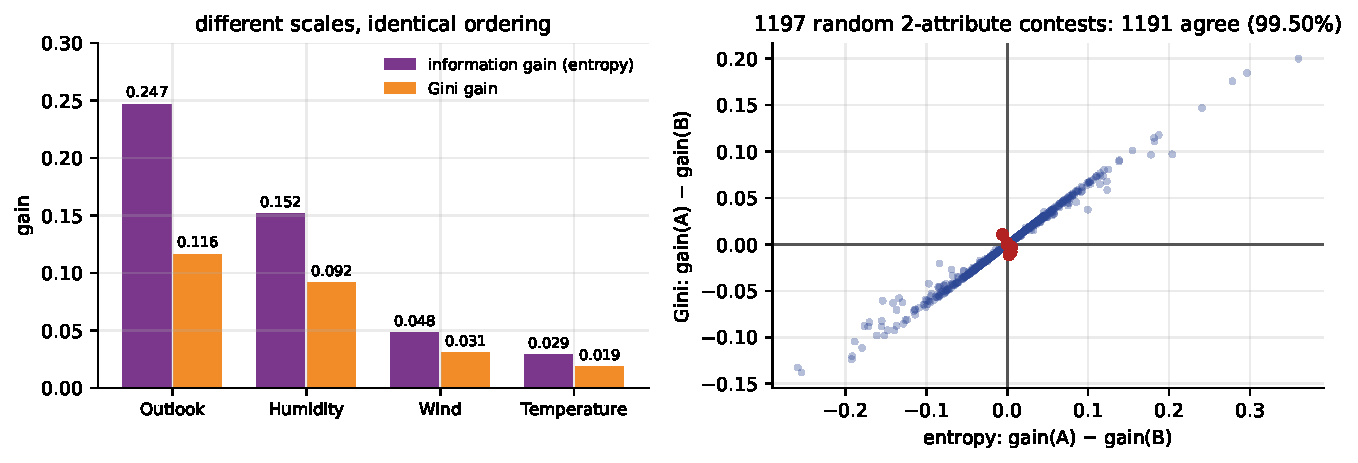
\includegraphics[width=0.90\textwidth]{giniig.pdf}
  \end{center}
  \begin{center}\small
    Left: the four tennis attributes scored both ways --- different heights,
    identical ordering. Right: two thousand random two-attribute contests,
    entropy's margin horizontally against Gini's vertically. Almost every
    point sits in the lower-left or upper-right quadrant, meaning the two
    agreed. \textbf{The red points --- $0.45\%$ of them --- all sit close to
    the origin}, where the two attributes were nearly tied anyway.
  \end{center}
\end{frame}

% =====================================================================
\section[Ratio]{Gain ratio, and the bias of information gain}
\label{sec:gainratio}

\begin{frame}[shrink=5]{Information gain has a flaw, and it is not subtle}
  \begin{exampleblock}{}
    \centering\large
    It systematically prefers attributes with \textbf{many values}.
  \end{exampleblock}
  \vspace{0.3em}
  \begin{columns}[T]
    \begin{column}{0.48\textwidth}
      \begin{block}{Why, in one sentence}
        An attribute that cuts the data into many small pieces produces
        children that are purer \emph{almost by accident}. In the limit, one
        value per row gives fourteen children of one row each, every one of
        them pure.
      \end{block}
    \end{column}
    \begin{column}{0.48\textwidth}
      \begin{alertblock}{And the tennis table has such a column}
        It is called \texttt{Day}. It has been sitting in the file since the
        first slide of the lecture, and nothing in the algorithm knows it is
        an identifier rather than an attribute.
      \end{alertblock}
    \end{column}
  \end{columns}
  \vspace{0.3em}
  \begin{center}
    \textbf{Predict first \#3: what information gain does \texttt{Day} score,
    and how does it compare with \texttt{Outlook}'s $0.246750$?}
  \end{center}
\end{frame}

\begin{frame}[fragile,shrink=8]{Predict first \#3 --- scoring the \texttt{Day} column}
Fourteen values in fourteen rows, so every child holds one row and has entropy
$0$. Therefore $\mathrm{Info}_{\texttt{Day}}(S) = \sum_v \tfrac{1}{14}\times 0
= 0$, and the gain is the whole of $H(S)$.
\vspace{0.2em}
\onslide<2->
\begin{outblk}
now score the Day column, which is a row identifier
Day has 14 distinct values in 14 rows
   Day = D1   1 row   H = 0.0000
   Day = D10  1 row   H = 0.0000
   Day = D11  1 row   H = 0.0000
   ... all 14 subsets have one row each, so every H = 0
Info_Day(S)  = 0.000000
Gain(S, Day) = 0.940286 - 0.000000 = 0.940286   <-- the largest possible
Gini gain(S, Day) = 0.459184   (Gini has exactly the same bias)
best real attribute:  Gain(S, Outlook) = 0.246750
Day beats it by a factor of 3.81
\end{outblk}
\onslide<3->
\begin{center}\small
  \textbf{The largest gain any attribute can possibly have}, $3.81\times$ the
  best real one --- and the Gini index has exactly the same problem, scoring
  the whole of $\mathrm{Gini}(S) = 0.459184$. This is not a defect of entropy.
  It is a defect of \emph{unnormalised impurity reduction}.
\end{center}
\end{frame}

\begin{frame}[fragile,shrink=8]{What ID3 does with it --- exactly what it is told}
\begin{outblk}
what happens if you let ID3 see the Day column
[9 Yes, 5 No  H=0.9403]  split on Day (gain 0.9403)
   Day=D1: [0 Yes, 1 No  H=0.0000] --> No
   Day=D10: [1 Yes, 0 No  H=0.0000] --> Yes
   Day=D11: [1 Yes, 0 No  H=0.0000] --> Yes
   ... (14 branches, one per row)
leaves 14, depth 1, conditions per rule 1
training rows reproduced: 14 of 14  (perfect)
a new row D15 (Sunny, Cool, Normal, Weak) matches 0 of the 14 rules
the 4-attribute tree classifies it as: Yes
\end{outblk}
\onslide<2->
\begin{alertblock}{Read the last two lines twice}
  \footnotesize A depth-1 tree with fourteen leaves, \textbf{perfect on the
  training set}, that \textbf{matches none of its own rules on a new day}.
  This is the cleanest demonstration of overfitting in the whole course: a
  model that is right about everything it has seen and has nothing whatever
  to say about anything else.
\end{alertblock}
\end{frame}

\begin{frame}[shrink=8]{The fix: divide by what the split itself costs}
  \begin{exampleblock}{C4.5: normalise by the entropy of the split itself, ignoring the labels}
    \[
      \mathrm{SplitInfo}_A(S) = -\sum_{v}\frac{|S_v|}{|S|}
         \log_2 \frac{|S_v|}{|S|},
      \qquad
      \mathrm{GainRatio}(S,A) = \frac{\mathrm{Gain}(S,A)}
                                     {\mathrm{SplitInfo}_A(S)}
    \]
  \end{exampleblock}
  A two-way even split has $\mathrm{SplitInfo} = 1$ and is not penalised at
  all. A fourteen-way split has $\log_2 14 = 3.807$ and is divided by nearly
  four.
  \begin{align*}
    \mathrm{SplitInfo}_{\texttt{Outlook}}
     &= -\tfrac{5}{14}\log_2\tfrac{5}{14} - \tfrac{4}{14}\log_2\tfrac{4}{14}
        - \tfrac{5}{14}\log_2\tfrac{5}{14} = 1.577406\\
    \mathrm{SplitInfo}_{\texttt{Humidity}}
     &= -\tfrac{7}{14}\log_2\tfrac{7}{14} - \tfrac{7}{14}\log_2\tfrac{7}{14}
        = 1.000000\\
    \mathrm{SplitInfo}_{\texttt{Day}} &= \log_2 14 = 3.807355
  \end{align*}
  \begin{center}\small
    \textbf{Predict first \#4: does dividing by that fix the \texttt{Day}
    problem?} $0.940286/3.807355$ against $0.246750/1.577406$ --- do the
    division before the next slide.
  \end{center}
\end{frame}

\begin{frame}[fragile,shrink=8]{Predict first \#4 --- the reveal}
\begin{outblk}
gain ratio = gain / split information
attribute      Gain      SplitInfo   GainRatio   gain rank  ratio rank
Outlook       0.246750   1.577406    0.156428      1          1
Temperature   0.029223   1.556657    0.018773      4          4
Humidity      0.151836   1.000000    0.151836      2          2
Wind          0.048127   0.985228    0.048849      3          3
information gain picks Outlook; gain ratio picks Outlook
\end{outblk}
\onslide<2->
\begin{outblk}
SplitInfo(Day) = log2(14) = 3.807355
GainRatio(Day) = 0.940286 / 3.807355 = 0.246966
that is a 73.7% cut, from 3.81x the best real attribute to 1.58x
but at 14 rows Day still ranks FIRST on gain ratio: 0.246966 vs Outlook 0.156428
\end{outblk}
\onslide<3->
\begin{alertblock}{Textbooks say gain ratio fixes the bias. On this table it does not}
  \footnotesize It \emph{reduces} it enormously --- a $73.7\%$ cut --- but
  $0.246966$ still beats $0.156428$, so \textbf{the identifier would still be
  chosen}. Do not claim otherwise in an answer script. Also notice what the
  correction did to the honest attributes: \texttt{Outlook} $0.156428$ against
  \texttt{Humidity} $0.151836$, a gap of $0.005$ where plain gain had $0.095$.
  The three-way split was penalised; the two-way one was not.
\end{alertblock}
\end{frame}

\begin{frame}[fragile,shrink=8]{Where the correction \emph{does} bite: more rows}
$\mathrm{SplitInfo}$ of an identifier is $\log_2 n$, which grows with the
table. Its gain is stuck at $H(S)$, which does not. So replicate the table.
\begin{outblk}
 copies  rows  Gain(RowID)  SplitInfo  GainRatio(RowID)  best real GR  Day wins?
      1    14     0.940286   3.807355          0.246966      0.156428   YES
      2    28     0.940286   4.807355          0.195593      0.156428   YES
      5    70     0.940286   6.129283          0.153409      0.156428   no
     10   140     0.940286   7.129283          0.131891      0.156428   no
     20   280     0.940286   8.129283          0.115667      0.156428   no
log2(rows) grows; the gain of a perfect identifier does not.
\end{outblk}
\onslide<2->
\begin{outblk}
   the 14-row table    gain picks Day      (14 leaves)   gain ratio picks Day      (14 leaves)
   5 copies, 70 rows   gain picks Day      (70 leaves)   gain ratio picks Outlook  (5 leaves)
\end{outblk}
\onslide<3->
\begin{center}\small
  At seventy rows it is unambiguous: information gain still builds the useless
  seventy-leaf identifier tree, and \textbf{gain ratio recovers the correct
  five-leaf tree}. That is the result to remember --- with the $n = 14$ caveat
  attached to it.
\end{center}
\end{frame}

\begin{frame}[shrink=6]{Drawn: the identifier, penalised}
  \begin{center}
    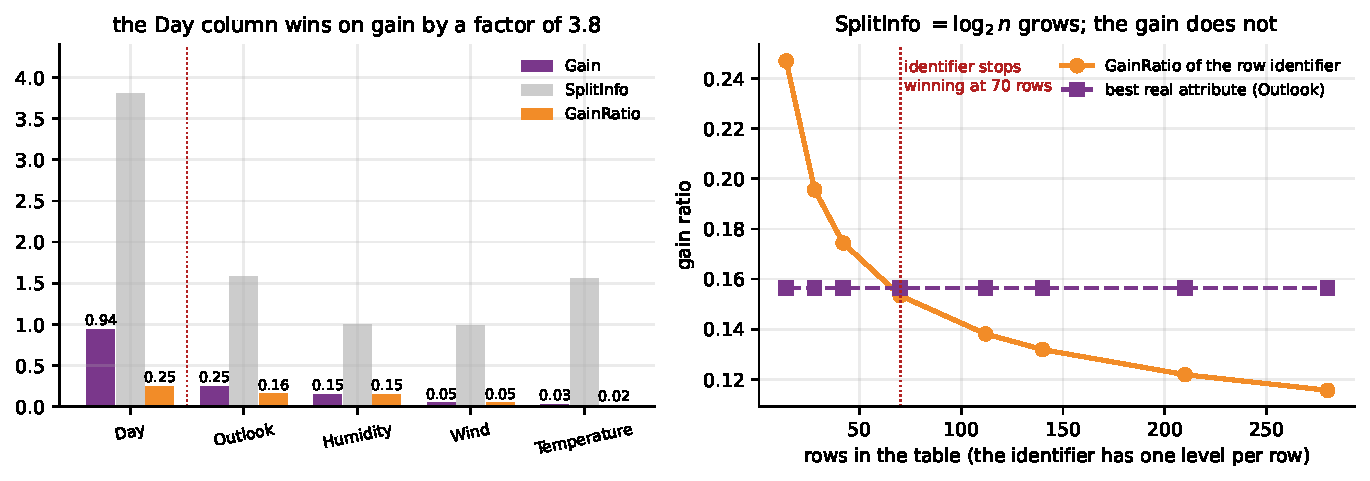
\includegraphics[width=0.92\textwidth]{gainratio.pdf}
  \end{center}
  \begin{center}\small
    Left: gain, split information and gain ratio for the four real attributes
    and \texttt{Day}. \texttt{Day}'s gain bar is the tallest possible; its
    split-information bar is $3.807$; dividing brings it down to $0.247$.
    Right: repeating the table so the identifier has more levels. Its gain
    ratio falls like $H(S)/\log_2 n$ while the best real attribute stays flat
    at $0.156$. \textbf{They cross at seventy rows.}
  \end{center}
\end{frame}

\begin{frame}[fragile,shrink=8]{Two honest footnotes before we leave this}
\begin{outblk}
the same identifier, one-hot encoded, given to scikit-learn
   4 attributes  (10 columns)     train 1.0000  depth 4  leaves 7  7-fold CV 0.6429
   + Day column  (24 columns)     train 1.0000  depth 3  leaves 5  7-fold CV 0.6429
   one-hot turns a 14-way question into 14 separate yes/no questions,
   so CART cannot isolate one row in a single split and the damage is
   milder than ID3's -- but the CV score is unchanged either way.
\end{outblk}
\onslide<2->
\begin{columns}[T]
  \begin{column}{0.5\textwidth}
    \begin{block}{C4.5 does not use the ratio blindly}
      \small It first discards any attribute whose \emph{plain} gain is below
      average, then maximises the ratio among the rest --- because dividing by
      a tiny $\mathrm{SplitInfo}$ can promote a useless near-constant
      attribute.
    \end{block}
  \end{column}
  \begin{column}{0.46\textwidth}
    \begin{alertblock}{The catastrophe is a \emph{multiway} one}
      \small Binary-split CART peels off one row at a time, so a one-hot
      identifier did not move the CV score here. The lesson survives either
      way, and it is short: \textbf{drop identifier columns before you fit
      anything.}
    \end{alertblock}
  \end{column}
\end{columns}
\end{frame}

% =====================================================================
\section[Scale]{Trees need no feature scaling}
\label{sec:scale}

\begin{frame}[fragile,shrink=10]{A split is a question about order, not magnitude}
Every question is ``is $x_j \le t$?''. Apply any strictly increasing $g$: then
$x_j \le t \iff g(x_j) \le g(t)$, so \textbf{the same rows go left} with a
different number printed on the node. Same partitions available, same tree.
\begin{outblk}
a tree needs no feature scaling: any increasing transform is a no-op
   tree  raw                              leaves 16 depth 6  test 0.906433  same predictions? True
   tree  StandardScaler                   leaves 16 depth 6  test 0.906433  same predictions? True
   tree  log1p (nonlinear, increasing)    leaves 16 depth 6  test 0.906433  same predictions? True
   tree  cube  (nonlinear, increasing)    leaves 16 depth 6  test 0.906433  same predictions? True
   tree  x -> -x (DECREASING)             leaves 19 depth 6  test 0.900585  same predictions? False
   the decreasing case: the SAME partitions are available, but the
   greedy search breaks its ties the other way round. Check the root:
   root feature raw 22 thr +106.1000 | negated 22 thr -106.1000 | same 2 groups? True
\end{outblk}
\onslide<2->
\begin{outblk}
   contrast: a distance-based model on the same splits
   5-NN  raw                                                  test 0.912281
   5-NN  StandardScaler                                       test 0.947368
   5-NN  log1p (nonlinear, increasing)                        test 0.935673
   5-NN  cube  (nonlinear, increasing)                        test 0.918129
   spread of the 4 tree scores 0.0000    spread of the 4 5-NN scores 0.0351
\end{outblk}
\onslide<3->
\begin{center}\small
  Not ``similar'': \textbf{identical predictions on every test row} under an
  affine rescaling, a logarithm and a cube. The fifth row looks like a
  counterexample and is not --- the root is the \emph{same} feature at the
  mirrored threshold, sending the same rows each way; the trees diverge lower
  down only through tie-breaking.
\end{center}
\end{frame}

\begin{frame}[shrink=8]{Drawn: the tree does not move, the neighbours do}
  \begin{center}
    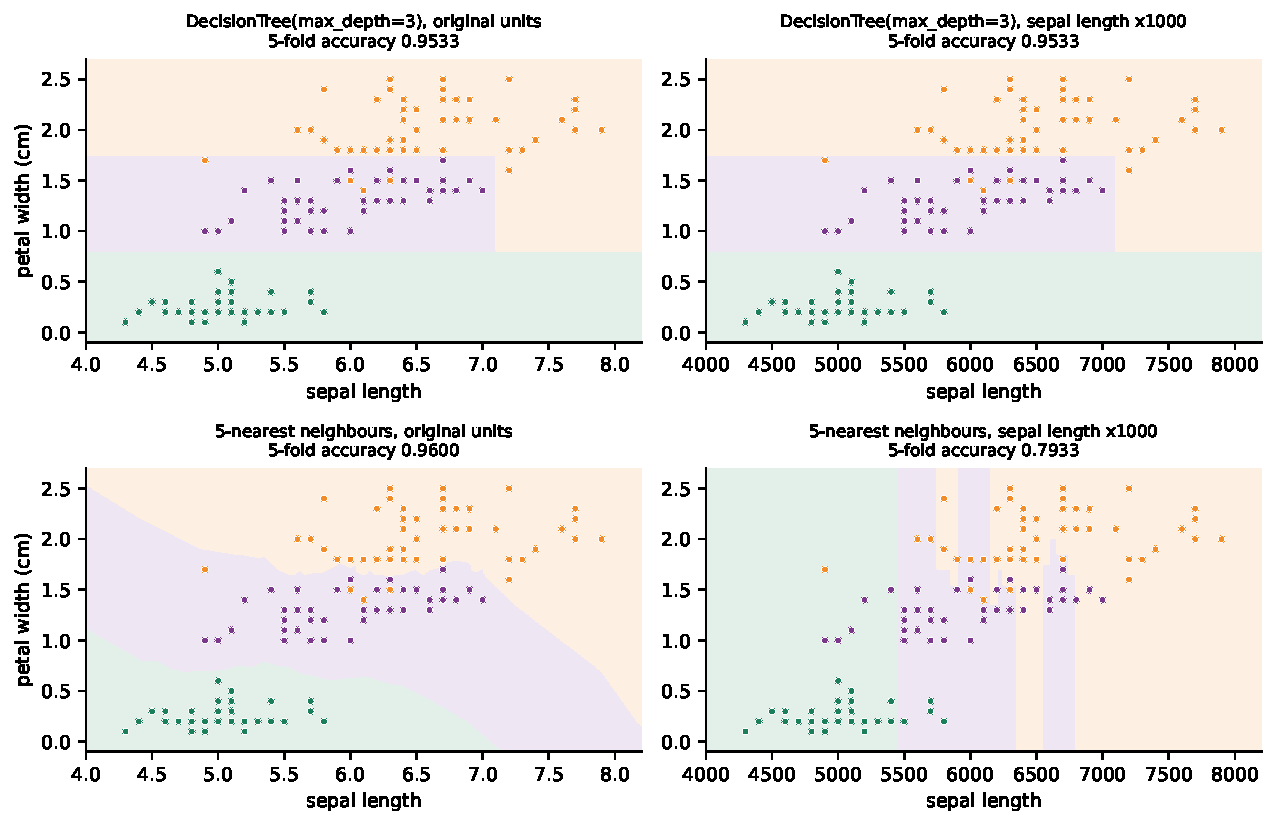
\includegraphics[width=0.78\textwidth]{invariance.pdf}
  \end{center}
  \begin{center}\small
    The right-hand column measures sepal length in units a thousand times
    smaller. Top: the tree's regions are the \emph{same picture} --- the axis
    numbers changed and nothing else --- and the accuracy is $0.9533$ in
    both. Bottom: $5$-NN collapses from $0.9600$ to $0.7933$. \textbf{It does
    not extend to rotations:} PCA before a tree mixes columns, so the
    questions are no longer about single features and the invariance is gone.
  \end{center}
\end{frame}

% =====================================================================
\section[Pruning]{Overfitting, and how to stop it}
\label{sec:prune}

\begin{frame}[fragile,shrink=8]{Predict first \#5 --- an unrestricted tree on real data}
ID3 and CART both stop only when a node is pure. Fit one to
\texttt{load\_breast\_cancer} with no limits at all.
\begin{center}
  \textbf{What training accuracy comes out --- and what does it cost?}
\end{center}
\vspace{0.2em}
\onslide<2->
\begin{outblk}
   breast_cancer  398 train rows, 171 test rows
   unrestricted: depth 6  leaves 16  train 1.0000  test 0.9064  gap +0.0936
   leaves holding a single training row: 5 of 16
\end{outblk}
\onslide<3->
\begin{outblk}
   600 rows, 20 features, 20% of the labels deliberately flipped
   unrestricted: depth 11  leaves 50  train 1.0000  test 0.6250  gap +0.3750
\end{outblk}
\onslide<4->
\begin{alertblock}{Training accuracy $1.0000$ from a tree is not an achievement}
  \footnotesize An unpruned tree reaches it \emph{every time}, as long as no
  two rows have identical features and different labels. On
  \texttt{breast\_cancer} the price is nine points; where a fifth of the
  labels are wrong by construction it is thirty-seven. \textbf{Five of the
  sixteen leaves hold a single patient each --- those are not rules, they are
  copies.}
\end{alertblock}
\end{frame}

\begin{frame}[fragile,shrink=10]{Pre-pruning: two dials, averaged over thirty splits}
\begin{outblk}
max_depth   leaves   train    test     gap
   1           2.0   0.9275   0.8977   +0.0298
   2           4.0   0.9563   0.9199   +0.0364
   3           7.7   0.9750   0.9232   +0.0518
   4          11.2   0.9874   0.9263   +0.0610
   5          14.0   0.9946   0.9312   +0.0634
   6          15.8   0.9986   0.9277   +0.0709
   8          16.5   1.0000   0.9271   +0.0729
   10         16.5   1.0000   0.9271   +0.0729
   None       16.5   1.0000   0.9271   +0.0729
min_samples_leaf   leaves   train    test     gap
   1                 16.5   1.0000   0.9271   +0.0729
   2                 14.9   0.9904   0.9275   +0.0629
   5                 11.4   0.9757   0.9339   +0.0418
   10                 8.3   0.9607   0.9209   +0.0399
   20                 6.3   0.9438   0.9205   +0.0233
   50                 4.9   0.9275   0.8977   +0.0298
\end{outblk}
\onslide<2->
\begin{center}\small
  Training accuracy climbs monotonically; test accuracy \textbf{rises, peaks
  and falls}. \texttt{max\_depth} $=5$ gives $0.9312$; \texttt{min\_samples\_leaf}
  $=5$ gives $0.9339$. \textbf{The train--test gap is the diagnostic, not the
  training score.}
\end{center}
\end{frame}

\begin{frame}[fragile,shrink=8]{Drawn: the same trade-off, and what noise does to it}
  \begin{center}
    
\includegraphics[width=0.94\textwidth]{overfit.pdf}
  \end{center}
\begin{outblk}
   max_depth 4       14.2 leaves  train 0.8330  test 0.7380  gap +0.0951
   max_depth 6       32.1 leaves  train 0.9122  test 0.7157  gap +0.1965
   max_depth 8       48.2 leaves  train 0.9641  test 0.7093  gap +0.2549
   max_depth None    62.1 leaves  train 1.0000  test 0.6920  gap +0.3080
\end{outblk}
\begin{center}\small
  On \texttt{breast\_cancer} the peak is shallow because the classes are well
  separated. With $20\%$ label noise it is dramatic: $0.7380$ at depth 4
  against $0.6920$ unrestricted, and the gap widens from $0.02$ to $0.31$.
\end{center}
\end{frame}

\begin{frame}[fragile,shrink=10]{Post-pruning: cost-complexity}
$R_\alpha(T) = R(T) + \alpha\,|\widetilde{T}|$ --- total impurity plus a price
per leaf. At $\alpha = 0$ the full tree wins; as $\alpha$ rises, whole
subtrees stop being worth their leaf count.
\begin{lstlisting}
path = DecisionTreeClassifier(random_state=0
                              ).cost_complexity_pruning_path(Xtr, ytr)
\end{lstlisting}
\begin{outblk}
   the path has 11 effective alphas, from 0.000000 to 0.026550
   alpha      leaves   train    5-fold CV   test
   0.002492     14   0.9975   0.9171      0.9064
   0.004902     10   0.9899   0.9121      0.9123
   0.008794      6   0.9774   0.9197      0.9181
   0.008992      5   0.9724   0.9197      0.9181
   0.019591      4   0.9623   0.9247      0.9006   <-- best CV
   0.025861      3   0.9322   0.9172      0.8889
   0.026550      2   0.9322   0.9172      0.8889
   chosen by cross-validation: alpha 0.019591, 4 leaves, test 0.9006
   unpruned: 16 leaves, test 0.9064
   pruning removed 12 of 16 leaves and changed the test score by -0.0058
   on breast_cancer the gain is in SIZE, not accuracy: report that.
\end{outblk}
\end{frame}

\begin{frame}[fragile,shrink=8]{Report the result you got, not the one you wanted}
  \begin{center}
    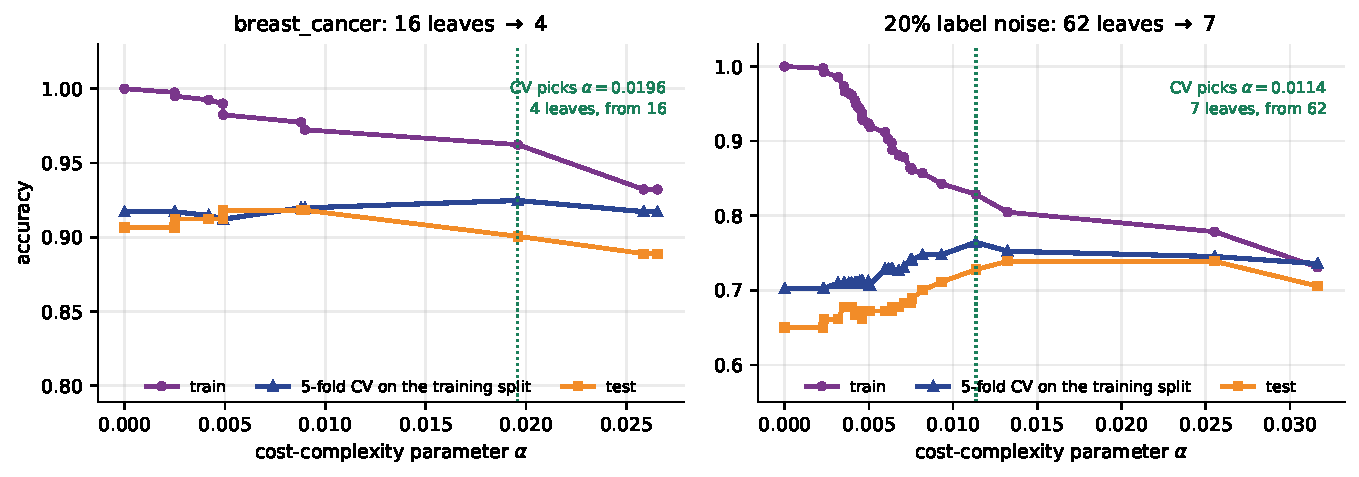
\includegraphics[width=0.82\textwidth]{ccp.pdf}
  \end{center}
\begin{outblk}
   unpruned      :  50 leaves  train 1.0000  CV 0.6917  test 0.6250
   best CV alpha 0.013805:   8 leaves  train 0.8500  CV 0.7444  test 0.7000
   pruning removed 42 of 50 leaves and bought +0.0750 of test accuracy
\end{outblk}
\begin{center}\small
  Same code, same procedure, different data. And choose $\alpha$ on the
  \textbf{blue} curve --- cross-validation inside the training split. The
  orange test curve is drawn so you can see whether it worked; picking the
  $\alpha$ that maximises \emph{it} is a leak.
\end{center}
\end{frame}

% =====================================================================
\section{Summary}
\label{sec:summary}

\begin{frame}[shrink=17]{Summary --- twelve lines}
  \begin{enumerate}\small
    \item A decision tree is a nested set of IF--THEN rules built greedily,
      top-down, one question at a time; with numeric features it is a
      partition into axis-parallel boxes.
    \item $H = -\sum p_i \log_2 p_i$ is $0$ for a pure node, $1$ for an even
      binary split, $\log_2 m$ for $m$ equal classes. Base two makes the unit
      a yes/no question.
    \item On the fourteen rows, $H(S) = \mathbf{0.940286}$ bits and
      $\mathrm{Gini}(S) = 0.459184$.
    \item The four gains: \texttt{Outlook} $\mathbf{0.246750}$,
      \texttt{Humidity} $0.151836$, \texttt{Wind} $0.048127$,
      \texttt{Temperature} $0.029223$. \texttt{Outlook} wins because it is
      the only attribute with a \textbf{pure child}.
    \item Recursing: \texttt{Sunny} is split perfectly by \texttt{Humidity}
      and \texttt{Rain} perfectly by \texttt{Wind}, both at gain $0.970951$.
      Depth 2, five leaves, \texttt{Temperature} never used.
    \item Five leaves means five rules and nine conditions, reproducing
      $14$ of $14$ rows. On iris, two rules predicting the same class let a
      condition go: five rules became four, still $146$ of $150$.
    \item Gini ranks the four attributes identically ($0.116327$ for
      \texttt{Outlook}) and agrees with entropy on $\mathbf{99.55\%}$ of two
      thousand contests --- but differed on $25\%$ of \texttt{breast\_cancer}
      bootstrap root splits, whose stumps still agreed on $98.4\%$ of rows.
    \item CART's best \emph{binary} cut on \texttt{Outlook} scores
      $0.102041$ against the multiway $0.116327$; on the tennis table it
      builds depth 4 and seven leaves where ID3 builds depth 2 and five.
    \item \texttt{Day} scores $\mathbf{0.940286}$, the maximum possible,
      $3.81\times$ \texttt{Outlook} --- and ID3 given it builds a depth-1
      fourteen-leaf tree that \textbf{matches none of its own rules on a new
      day}.
    \item Gain ratio divides by $\log_2 14 = 3.807355$, a $73.7\%$ cut, but
      $0.246966$ still beats $0.156428$ at $n=14$. At seventy rows gain ratio
      recovers the five-leaf tree while plain gain builds a seventy-leaf one.
    \item A tree is invariant to any monotone transform: raw, standardised,
      $\log$ and cubed gave \textbf{identical predictions}, $16$ leaves, test
      $0.906433$; the same transforms moved $5$-NN over $0.0351$.
    \item Unrestricted trees hit train $\mathbf{1.0000}$ every time, costing
      $0.0936$ on \texttt{breast\_cancer} and $0.3750$ under $20\%$ label
      noise. Cost-complexity pruning cut $16$ leaves to $4$ for $-0.0058$ ---
      and $50$ leaves to $8$ for $\mathbf{+0.0750}$. Report both.
  \end{enumerate}
\end{frame}

\begin{frame}[shrink=3]{Before the next lecture}
  \begin{columns}[T]
    \begin{column}{0.48\textwidth}
      \begin{block}{Read}
        \texttt{notes.pdf} --- the full derivation of entropy, every gain
        computed twice, the ID3 recursion in detail, and \textbf{practice
        questions with worked solutions}.
      \end{block}
      \begin{block}{Do}
        Reproduce the entire fourteen-row calculation with a pen and no
        calculator beyond $\log_2$: $H(S)$, four gains, both recursions, the
        five rules. \textbf{Then do it again for the \texttt{Day} column} and
        say in one sentence why the answer is a disaster.
      \end{block}
    \end{column}
    \begin{column}{0.48\textwidth}
      \begin{exampleblock}{Next: more classifiers}
        Trees are one shape of decision boundary. The next lectures build
        others, and the vocabulary of this one --- greedy, impurity,
        overfitting, the train--test gap --- carries straight across.
      \end{exampleblock}
      \begin{alertblock}{A habit to start now}
        Before you fit anything, \textbf{look at the columns and delete the
        identifiers}. Row numbers, ticket numbers, patient IDs, timestamps
        used as labels. Information gain will happily pick every one of them.
      \end{alertblock}
    \end{column}
  \end{columns}
  \begin{center}
    \small Materials: \texttt{\AMLRepoURL}
  \end{center}
  \slidesources{\AMLUnitVISources}
\end{frame}

\end{document}
